\documentclass[a4paper]{CSMakotoTechnicalReport}

\usepackage[spanish, es-noshorthands]{babel}
\usepackage{csquotes} 
\usepackage{caption}
\usepackage{xcolor}
\usepackage{xurl}
\usepackage{amssymb}

%----------------------------------------------------------------------------------------
%   REPORT INFORMATION
%----------------------------------------------------------------------------------------

\reporttitle{Servidor POP3: \textit{nano-pop}}

\reportsubtitle{Memoria y manual del proyecto}

\reportauthors{Andrés Súnico Sánchez}

\reportdate{\today}

%----------------------------------------------------------------------------------------

\begin{document}

%----------------------------------------------------------------------------------------
%   PORTADA
%----------------------------------------------------------------------------------------

\thispagestyle{empty} % Suppress headers and footers on this page

\vspace*{0.05\textheight} % Vertical whitespace

{\large\raggedright\reportdate\par} % Report date

\vspace{0.01\textheight} % Vertical whitespace

{\fontsize{32pt}{34pt}\selectfont\raggedright\textbf{\reporttitle}\par} % Report title

\vspace{0.01\textheight} % Vertical whitespace

{\Large\raggedright\textit{\textbf{\reportsubtitle}}\par} % Subtitle

\vspace{0.01\textheight} % Vertical whitespace

{\large\raggedright\reportauthors\par} % Report authors, group or department

\vspace{0.26\textheight} % Vertical whitespace

%----------------------------------------------------------------------------------------

\begin{multicols}{2} % Begin two column mode

%----------------------------------------------------------------------------------------
%   ÍNDICE
%----------------------------------------------------------------------------------------

\setcounter{tocdepth}{2}
\tableofcontents

%----------------------------------------------------------------------------------------
%   INTRODUCCIÓN
%----------------------------------------------------------------------------------------

\section*{Introducción}

El desarrollo de \textit{nano-pop} ha priorizado ante todo la corrección. Un servidor \texttt{POP3} no es una aplicación aislada e independiente, sino que está diseñado para interactuar con otros sistemas que esperan un cumplimiento riguroso del protocolo.

En este contexto, el uso de \textit{Haskell} resulta especialmente valioso. Un buen diseño en este lenguaje no sólo permite garantizar las invariantes del sistema con facilidad, sino también hacer que los estados ilegales sean directamente irrepresentables.

Para ello, se han empleado patrones como \textit{typestate} y \textit{resource acquisition}, que no sólo aportan a la aplicación una robustez difícil de alcanzar en otros lenguajes, sino que también aumentan la claridad del código.

Esta prioridad por la corrección también se ha reflejado en la validación del sistema, mediante \textit{unit tests} sobre los módulos más propensos a errores, pruebas de \textit{fuzzing} sobre el \textit{parser} y tests de integración con clientes \texttt{POP3} reales.

Además, se ha desarrollado un \textit{script} adicional para facilitar la configuración del servidor, así como la gestión local de usuarios y mensajes.

%----------------------------------------------------------------------------------------

\end{multicols} % Ends two column mode
\newpage
\setcounter{page}{1}

%----------------------------------------------------------------------------------------
%   EL PROTOCOLO POP3
%----------------------------------------------------------------------------------------

\section{El protocolo POP3}

Para entender \texttt{POP3}, primero hay que hablar del \textit{Simple Mail Transport Protocol} o \texttt{SMTP}, que gobierna la comunicación \textit{e-mail}. Imaginemos que Alice desea enviarle un correo a su amigo Bob. El proceso es el siguiente:

\begin{enumerate}
    \item Alice escribe el correo y se lo entrega a su agente \textit{e-mail} para que lo envíe.
    \item El agente de Alice utiliza \texttt{SMTP} para enviar el mensaje a su servidor \textit{mail}, dónde se deposita en una cola.
    \item El servidor \textit{mail} de Alice abre una conexión \texttt{TCP} al servidor \textit{mail} de bob y el correo se envía utilizando \texttt{SMTP}, dónde se deposita en el buzón de Bob.
\end{enumerate}

\begin{figure}[h]
  \centering
  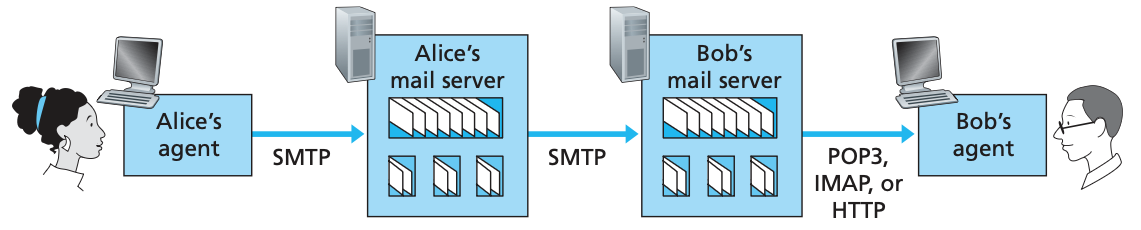
\includegraphics[width=0.94\textwidth]{images/mail-communication.png}
  \caption{Protocolos \textit{email} y sus entidades~\cite{kurose2013}.}
  \label{fig:mail-communication}
\end{figure}

Podría pensarse que bastaría con utilizar \texttt{SMTP} para entregar el correo al dispositivo de Bob. Sin embargo, \texttt{SMTP} es un protocolo \textit{push}: quien inicia la conexión es quien envía los datos. Cuando Bob quiere consultar su buzón es él quien toma la iniciativa, no su servidor, por lo que no se puede utilizar \texttt{SMTP}.

La solución llegó en los años 90 con los protocolos de acceso \textit{mail}, diseñados para transferir correos desde el servidor hasta el dispositivo del usuario. Uno de ellos es el \textit{Post Office Protocol}, conocido como \texttt{POP3}~\cite{rfc1939}.

%----------------------------------------------------------------------------------------

\subsection{Descripción básica}

El servidor inicia el servicio \texttt{POP3} escuchando por el puerto \texttt{TCP} 110. Una vez se establece conexión con un cliente, el servidor envía un saludo. A partir de aquí, el cliente y servidor intercambiarán comandos y respuestas hasta que la conexión se cierra o interrumpe.

Un comando empieza por una \textit{keyword} que lo identifica, opcionalmente seguida de uno o más argumentos. Por otro lado, una respuesta consiste en un indicador positivo (\texttt{+OK}) o negativo (\texttt{-ERR}), seguido de información adicional.

Una sesión \texttt{POP3} atraviesa múltiples estados durante su ciclo de vida. Tras el saludo inicial, comienza la fase de autorización, en la que el cliente debe identificarse. Durante esta fase hay tres comandos disponibles:

\begin{tabular}{ll}
    \texttt{\textbf{USER name}} & El cliente especifica su nombre de usuario.       \\
    \texttt{\textbf{PASS pass}} & El cliente especifica su contraseña.              \\
    \texttt{\textbf{QUIT}}      & El cliente aborta la sesión sin realizar cambios. \\
\end{tabular}

Si se autoriza al cliente, el servidor adquiere exclusivamente los recursos asociados a su buzón y se entra en la fase de transacción. En esta fase, el cliente realiza peticiones y acciones sobre su buzón. Los comandos disponibles son:

\begin{tabular}{ll}
    \texttt{\textbf{STAT}}          & El servidor responde con el número de mensajes y la suma de sus tamaños.          \\
    \texttt{\textbf{LIST [msg]}}    & El servidor responde con información sobre el índice y tamaño de mensajes.        \\
    \texttt{\textbf{UIDL [msg]}}    & El servidor responde con información sobre el índice e identificador de mensajes. \\
    \texttt{\textbf{RETR msg}}      & El servidor responde con el contenido del mensaje provisto.                      \\
    \texttt{\textbf{DELE msg}}      & El servidor marca como borrado el mensaje provisto.                               \\
    \texttt{\textbf{RSET}}          & El servidor restaura todos los mensajes marcados como borrados.                   \\
    \texttt{\textbf{NOOP}}          & El servidor no hace nada y responde positivamente.                                \\
    \texttt{\textbf{QUIT}}          & El cliente termina la sesión, que pasa a la fase de actualización.                \\
\end{tabular}

Una vez el servidor recibe el comando \texttt{QUIT}, la sesión entra en la fase de actualización. En esta última fase, el servidor libera todos los recursos adquiridos, guardando los cambios realizados, y cierra la conexión \texttt{TCP}.

\begin{figure}[H]
\centering
\begin{minipage}[t]{0.55\textwidth}

\subsection{Formato Maildir}

\medskip
Aunque el \texttt{RFC} de \texttt{POP3} no especifica cómo deben almacenarse los mensajes, uno de los formatos más extendidos es \textit{Maildir}~\cite{maildir}, que organiza los mensajes directamente mediante el sistema de ficheros.

\medskip
Cada usuario dispone de un directorio \textit{mail} con dos subdirectorios: \texttt{new} para mensajes no leídos y \texttt{cur} para los ya leídos. El estado de cada mensaje queda codificado en su propio nombre: los no leídos siguen el esquema \texttt{<time>.<pid>.<hostname>}, y los leídos añaden el sufijo \texttt{:2,} seguido de una lista de \textit{flags} en forma de carácteres. 

\medskip
Además, \textit{Maildir} simplifica la sincronización mediante un fichero \texttt{.lock} en el buzón del usuario, garantizando que no existan dos sesiones simultáneas sobre el mismo buzón.

\medskip
Cuando un usuario recibe un correo, este se deposita en \texttt{new}. Al leerlo con \texttt{RETR} y completar la fase de actualización, el servidor lo traslada a \texttt{cur} añadiendo el sufijo \texttt{:2,S}, dónde la bandera \texttt{S} (\textit{Seen}) indica que el mensaje ha sido leído.

\medskip
En esta práctica se emplea una variante adaptada a usuarios virtuales: en lugar de usar los directorios \texttt{home} del sistema, todos los buzones se agrupan bajo un directorio raíz común \texttt{npop/}, junto a un fichero \texttt{shadow} con las credenciales en forma de pares \texttt{<usuario>:<hash>}.
\end{minipage}
\hfill
\begin{minipage}[t]{0.35\textwidth}

\begin{lstlisting}[language = {}, frame=none, numbers=none, basicstyle=\footnotesize]
/home/user/Maildir/
+-- cur/
|   +-- 1.1.localhost:2,S
|   +-- 3.1.localhost:2,S
|   +-- 4.1.localhost:2,S
|
+-- new/
    +-- 5.1.localhost
    +-- 6.1.localhost
\end{lstlisting}
\captionof{lstlisting}{Maildir tradicional}

\begin{lstlisting}[language = {}, frame=none, numbers=none]
npop/
+-- bob/
|   +-- cur/
|   |   +-- 3.1.localhost:2,S
|   |   +-- 4.1.localhost:2,S
|   |
|   +-- new/
|       +-- 5.1.localhost
|
+-- alice/
|   +-- cur/
|   |   +-- 1.1.localhost:2,S
|   |   +-- 2.1.localhost:2,S
|   |
|   +-- new/
|       +-- 6.1.localhost
|
+-- shadow
\end{lstlisting}
\captionof{lstlisting}{Maildir modificado}

\end{minipage}
\end{figure}

%----------------------------------------------------------------------------------------
%   DISEÑO DE LA APLICACIÓN
%----------------------------------------------------------------------------------------

\vspace{-10pt}
\begin{figure}[H]
\centering
\begin{minipage}[t]{0.42\textwidth}
\vspace{0pt}
\section{Diseño de la aplicación}
La aplicación sigue un esquema típico de servidor, pero con un giro funcional. La aplicación comienza escuchando por el puerto 110, esperando algún cliente.

\medskip
Una vez se recibe una conexión, se crea un \textit{thread} de sesión para manejar el cliente, mientras que el \textit{thread} principal vuelve a ponerse a escuchar por el puerto.

\medskip
Por su parte, el \textit{thread} de sesión se ocupa de responder todos los \textit{queries} del cliente, cambiando su comportamiento dependiendo de la fase \texttt{POP3} en la que se encuentre.

\medskip
Las distintas fases de una sesión, como se desarrolla más adelante, se han modelado como un autómata finito.
\end{minipage}
\hfill
\begin{minipage}[t]{0.50\textwidth}
\vspace{0pt}
    \centering
    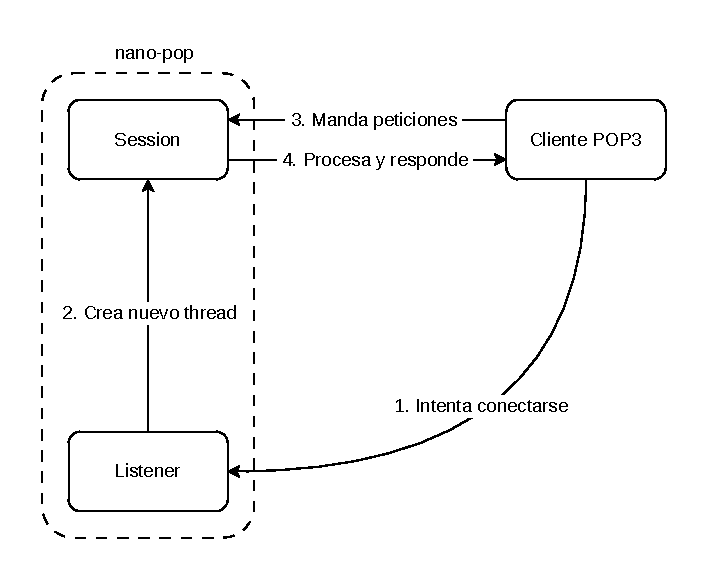
\includegraphics[width=\textwidth]{images/scheme.pdf}
    \captionof{figure}{Esquema de la aplicación.}
    \label{fig:scheme}
\end{minipage}
\end{figure}

\vspace{-10pt}
La aplicación se apoya además en varios componentes auxiliares que abstraen gran parte de la complejidad de bajo nivel. Entre ellos, destaca el módulo de red, que se encarga de abstraer llamadas al sistema como \texttt{socket} o \texttt{listen} mediante primitivas de más alto nivel.

Entre sus funciones destacan \texttt{withListener} y \texttt{forkClient}, que se encargan de adquirir, respectivamente, \textit{sockets} de escucha y de conexión, y que además gestionan automáticamente la liberación de recursos. También es interesante la función de orden superior \texttt{retryBackoff}, que permite reintentar operaciones bloqueantes aplicando una estrategia de \textit{exponential backoff}.

No obstante, dado el alcance y la extensión del proyecto, esta memoria se centrará principalmente en los módulos que forman parte del flujo principal de ejecución.

%----------------------------------------------------------------------------------------

\subsection{Gestión de errores}

La gestión de errores es un aspecto fundamental en el desarrollo de sistemas robustos y fiables. En el contexto de un servidor, una excepción no controlada puede provocar la terminación completa del proceso, dejando el servicio inaccesible para todos los clientes conectados. Este problema resulta especialmente relevante en \textit{Haskell}, ya que cualquier operación dentro de la mónada \texttt{IO} puede lanzar excepciones en tiempo de ejecución.

En primer lugar, para enrriquecer las excepciones que, sobretodo en llamadas de bajo nivel como \texttt{accept} o \texttt{bind}, tienen mensajes muy poco informativos, se ha definido el tipo el \texttt{SysErr}. Este \textit{wrapper} se encarga de envolver el tipo \texttt{IOException} y dotarlo de contexto adicional:

\vspace{-20pt}
\begin{minipage}[t]{0.40\textwidth}
\begin{lstlisting}[language=Haskell, frame=none, numbers=none, basicstyle=\footnotesize]
-- Etiqueta que identifica la operación
-- que lanzó la excepción, con campos
-- adicionales para aportar contexto.
data Oper
  = OpAddrInfo            -- getAddrInfo
  | OpOpenSock SockAddr   -- openSocket
  ... 
  | OpClose FilePath      -- closeFd
  | OpUser                -- custom
\end{lstlisting}
\vspace{-4pt}
\captionsetup{type=lstlisting}
\caption{Definición de Oper.}
\end{minipage}
\hfill
\begin{minipage}[t]{0.55\textwidth}
\begin{lstlisting}[language=Haskell, frame=none, numbers=none, basicstyle=\footnotesize]
-- Wrapper de 'IOException' que aporta
-- información adicional mediante 'Oper'.
data SysErr = SysErr
  { seOper :: Oper          -- Operación intentada
  , seExcp :: IOException   -- Excepción lanzada
  }

-- Implementación de 'Exception' por 'SysErr'
instance Exception SysErr
\end{lstlisting}
\vspace{-4pt}
\captionsetup{type=lstlisting}
\caption{Definición de SysErr.}
\end{minipage}
\vspace{6pt}

En cuanto al tratamiento de las excepciones, se distinguen dos clases: 

\begin{itemize}
    \item \textbf{Previsibles:} Aquellas que el cliente es capaz de provocar, como introducir un nombre de usuario inexistente o desconectarse matando el proceso en lugar de usando el comando \texttt{QUIT}.
    \item \textbf{Internas:} Que dependen únicamente del estado del servidor e indican un error en el código, en la configuración del servidor, o un fallo del sistema operativo.
\end{itemize}

Las excepciones previsibles se gestionan de forma explícita y no se dejan propagar, sino que se capturan en el punto donde se producen. En cambio, las excepciones internas sí se permiten propagar hasta el \textit{top-level}. Una vez ahí, se registra el error mediante la función \texttt{emit} del módulo de \textit{logging} y el sistema continúa su ejecución. Esta estrategia es segura gracias al uso de \texttt{bracket} para la gestión de recursos, que los libera automáticamente.

\vspace{-4pt}
\begin{minipage}[t]{0.55\textwidth}
\vspace{0pt}
En el Listing \ref{lst:open-excl} se ve la aplicación de estas pautas. La función \texttt{openExcl} intenta abrir un fichero en modo exclusivo, por lo que si éste ya existe se lanza una excepción.

\medskip
Esta situación puede producirse de forma esperada, por ejemplo si un cliente intenta iniciar dos sesiones concurrentes con el mismo usuario. En ese caso, la excepción se captura y se gestiona de forma controlada. En cambio, cualquier otro tipo de error se considera un fallo del sistema operativo y se propaga.
\end{minipage}
\hfill
\begin{minipage}[t]{0.40\textwidth}
\vspace{0pt}
\begin{lstlisting}[language=Haskell, frame=none, numbers=none, basicstyle=\footnotesize, aboveskip=0pt]
-- Intenta abrir el fichero con el path
-- provisto en modo exclusivo.
openExcl :: FilePath -> IO (Maybe Fd)
openExcl path =
  (Just <$> tryOpen path ReadWrite flags)
    `catch` \(err :: SysErr) ->
      case classify err of
        AlreadyExists -> pure Nothing
        _             -> throwIO err
\end{lstlisting}
\vspace{-4pt}
\captionsetup{type=lstlisting}
\caption{Manejo de excepciones en openExcl.}
\label{lst:open-excl}
\end{minipage}

%----------------------------------------------------------------------------------------

\subsection{Entorno y configuración}

A lo largo de la ejecución del servidor se tienen que arrastrar dos estructuras:

\begin{itemize}
    \item \textbf{Config:} Contiene la configuración del servidor, leída del fichero \texttt{config.toml}.
    \item \textbf{Shadow:} Mapea los usuarios del servidor a sus \textit{hashes}, para poder autenticarlos.
\end{itemize}

Ambas se cargan una única vez al inicar el servidor y nunca son modificadas. Por tanto, en vez de hacer que todas las funciones tomen ambos como argumentos y los devuelvan para preservarlos, se utiliza la mónada \texttt{ReaderT}:

\vspace{-20pt}
\begin{minipage}[t]{0.40\textwidth}
\begin{lstlisting}[language=Haskell, frame=none, numbers=none, basicstyle=\footnotesize]
-- Agrupa la configuración del servidor y
-- el fichero shadow en un único entorno.
data AppEnv = AppEnv
  { config :: Config
  , shadow :: Shadow
  }
\end{lstlisting}
\vspace{-4pt}
\captionsetup{type=lstlisting}
\caption{Entorno de la aplicación.}
\end{minipage}
\hfill
\begin{minipage}[t]{0.55\textwidth}
\begin{lstlisting}[language=Haskell, frame=none, numbers=none, basicstyle=\footnotesize]
-- Añade el entorno de lectura 'AppEnv' a la mónada 'IO'.
type App = ReaderT AppEnv IO

-- Desenvuelve una acción 'App' en una 'IO'.
runApp :: App a -> AppEnv -> IO a
runApp = runReaderT
\end{lstlisting}
\vspace{-4pt}
\captionsetup{type=lstlisting}
\caption{Definición de la mónada App.}
\end{minipage}

%----------------------------------------------------------------------------------------

\subsection{Flujo de una petición}
El procesamiento de una petición comienza con la reconstrucción del mensaje recibido desde la red. Como los datos no llegan de forma atómica, sino fragmentados en \textit{chunks} de \textit{bytes}, es necesario ir ensamblándolos progresivamente hasta obtener un mensaje completo, delimitado por \texttt{CRLF}. A partir de ese mensaje crudo, el servidor realiza una fase de \textit{parsing} para identificar el comando recibido, transformándolo en el tipo algebraico \texttt{Query}.

Cada comando puede interpretarse identificando primero el nombre de la operación y aplicando después un \textit{parser} específico para sus argumentos. De este modo, tras extraer el primer \textit{token} del mensaje, que determina el tipo de comando recibido, el servidor consulta el mapa \texttt{parsers} para obtener su correspondiente decodificador.

\vspace{-24pt}
\begin{minipage}[t]{0.54\textwidth}
\begin{lstlisting}[language=Haskell, frame=none, numbers=none, basicstyle=\footnotesize]
-- Representa una petición correcta
data Query
  = User ByteString       -- USER nombre
  | Pass ByteString       -- PASS contraseña
  | Stat                  -- STAT
  | List (Maybe MsgNo)    -- LIST [número]
  | Uidl (Maybe MsgNo)    -- UIDL [número]
  | Retr MsgNo            -- RETR número
  | Dele MsgNo            -- DELE número
  | Noop                  -- NOOP
  | Rset                  -- RSET
  | Quit                  -- QUIT

-- Parser de los argumentos de una petición
type QueryParser = [ByteString] -> Maybe Query
\end{lstlisting}
\vspace{-4pt}
\captionsetup{type=lstlisting}
\caption{Definición de Query y QueryParser.}
\end{minipage}
\hfill
\begin{minipage}[t]{0.45\textwidth}
\begin{lstlisting}[language=Haskell, frame=none, numbers=none, basicstyle=\footnotesize]
-- Mapea cada comando POP3
-- a un parser de sus argumetos
parsers :: [(ByteString, QueryParser]
parsers = 
  [ ("USER", parseString   User)
  , ("PASS", parseString   Pass)
  , ("LIST", parseOptMsgNo List)
  , ("UIDL", parseOptMsgNo Uidl)
  , ("RETR", parseMsgNo    Retr)
  , ("DELE", parseMsgNo    Dele)
  , ("STAT", parseVoid     Stat)
  , ("NOOP", parseVoid     Noop)
  , ("RSET", parseVoid     Rset)
  , ("QUIT", parseVoid     Quit)
  ]
\end{lstlisting}
\vspace{-4pt}
\captionsetup{type=lstlisting}
\caption{Mapa de comandos a parsers.}
\end{minipage}
\vspace{2pt}

Una vez construido el \texttt{Query}, este es procesado para producir una respuesta adecuada y, si la petición lo indica, realizar las acciones necesarias en el buzón del cliente. Una respuesta correcta se representa con el tipo algebraico \texttt{Reply} y su procesado depende de la fase en la que se encuentre la sesión, de lo que se hablará más adelante.

La última etapa consiste en serializar dicha respuesta y convertirla nuevamente en una secuencia de bytes para ser transmitida por la red. Una vez enviada, el cliente puede emitir una nueva petición, reiniciando el ciclo.

\vspace{-24pt}
\begin{minipage}[t]{0.40\textwidth}
\begin{lstlisting}[language=Haskell, frame=none, numbers=none, basicstyle=\footnotesize]
-- Representa una respuesta
-- positiva o negativa a un 'Query'
data Reply
  = RepHelo
  | RepUser
  | RepPass PassReply
  ...
  | RepQuit QuitReply
  | RepExcp
  | RepErr SessionErr
\end{lstlisting}
\vspace{-4pt}
\captionsetup{type=lstlisting}
\caption{Definición de Reply.}
\end{minipage}
\hfill
\begin{minipage}[t]{0.55\textwidth}
\begin{lstlisting}[language=Haskell, frame=none, numbers=none, basicstyle=\footnotesize]
class Serialize a where
  -- Serializa el tipo 'a' en una cadena de bytes
  serialize :: MonadIO f => a -> f ByteString

-- Serialización de una 'Reply'
instance Serialize Reply where
  serialize = \case
    RepPass pass -> serialize pass
    RepStat stat -> serialize stat
    ...
\end{lstlisting}
\vspace{-4pt}
\captionsetup{type=lstlisting}
\caption{Clase Serialize e instancia de Reply.}
\end{minipage}
\vspace{2pt}

En conjunto, el flujo completo puede entenderse como una composición de transformaciones sobre valores en la mónada \texttt{App}, un modelo que encaja de forma natural con el estilo funcional de \textit{Haskell}. Esto se aprecia especialmente en las funciones \texttt{recvQuery} y \texttt{sendReply}, definidas para abstraer aún más la lógica de comunicación.

\vspace{-24pt}
\begin{minipage}[t]{0.47\textwidth}
\begin{lstlisting}[language=Haskell, frame=none, numbers=none, basicstyle=\footnotesize]
-- Recibe y decodifica un query del cliente.
recvQuery :: Connection -> App QueryResult
recvQuery conn = parseQuery <$> recvClient conn
\end{lstlisting}
\vspace{-4pt}
\captionsetup{type=lstlisting}
\caption{Definición de recvQuery.}
\end{minipage}
\hfill
\begin{minipage}[t]{0.52\textwidth}
\begin{lstlisting}[language=Haskell, frame=none, numbers=none, basicstyle=\footnotesize]
-- Serializa y envía una respuesta al cliente.
sendReply :: Connection -> Reply -> App ()
sendReply conn = sendClient conn <=< serialize
\end{lstlisting}
\vspace{-4pt}
\captionsetup{type=lstlisting}
\caption{Definición de sendReply.}
\end{minipage}
\vspace{5pt}

\begin{figure}[H]
    \centering
    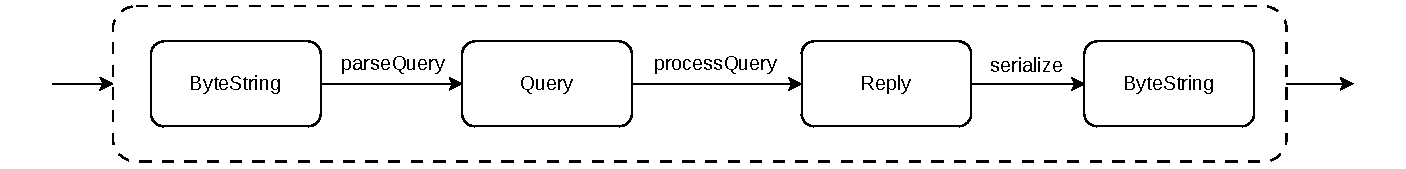
\includegraphics[width=\textwidth, trim={0.8cm 0cm 0.8cm 0cm}, clip]{images/pipeline.pdf}
    \captionof{figure}{Transformaciones de una petición.}
    \label{fig:pipeline}
\end{figure}

%----------------------------------------------------------------------------------------

\subsection{Autómata de una sesión}

Los estados de una sesión \texttt{POP3} pueden representarse de forma natural mediante un autómata finito determinista. El sistema inicia en la fase de autorización, desde la cual la sesión puede finalizar sin cambios con el comando \texttt{QUIT}, o avanzar a la fase de transacción tras una autenticación correcta mediante usuario y contraseña.

En la fase de transacción, el cliente puede ejecutar comandos sobre el buzón, y la única transición de salida posible es mediante \texttt{QUIT}, que conduce a la fase de actualización. En este último estado, se consolidan los cambios realizados y se termina la sesión.

\vspace{-8pt}
\begin{figure}[H]
    \centering
    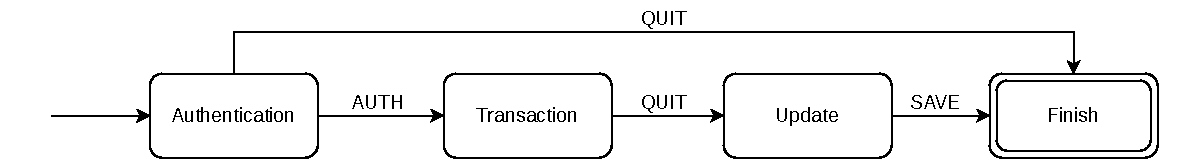
\includegraphics[width=\textwidth, trim={0.8cm 0cm 0.7cm 0cm}, clip]{images/automaton-pop3.pdf}
    \captionof{figure}{Autómata de una sesión \texttt{POP3}.}
    \label{fig:automaton-pop3}
\end{figure}
\vspace{-8pt}

Un autómata finito, en esencia, impone restricciones. Por ejemplo, en el autómata de una sesión \texttt{POP3} se impone que la única manera de llegar a la fase de actualización es a través de la de transacción. En \textit{Haskell}, estas normas se pueden imponer con el sistema de tipos utilizando el patrón \textit{typestate}.

En primer lugar hay que definir los estados del autómata. Aunque tradicionalmente pueden representarse usando \textit{phantom types}, la extensión \textit{DataKinds} permite agruparlos en un único tipo. Posteriormente, mediante un \texttt{GADT}, se puede construir un tipo indexado por el estado en el que se encuentre la sesión~\cite{sidorenko2026gadts}.

Además de los tres estados definidos por \texttt{POP3}, se añade un estado intermedio de verificación que valida los credenciales del usuario, avanzando al estado de transacción si son correctos, o volviendo atrás en caso contrario. 

\vspace{-20pt}
\begin{minipage}[t]{0.40\textwidth}
\begin{lstlisting}[language=Haskell, frame=none, numbers=none, basicstyle=\footnotesize]
-- Representa los distintos estados
-- que puede asumir el autómata
data PhaseTag
  = Auth        -- Autenticación
  | Verif       -- Verificación
  | Trans       -- Transacción
  | Update      -- Actualización
\end{lstlisting}
\vspace{-4pt}
\captionsetup{type=lstlisting}
\caption{Defnición de los estados.}
\end{minipage}
\hfill
\begin{minipage}[t]{0.55\textwidth}
\begin{lstlisting}[language=Haskell, frame=none, numbers=none, basicstyle=\footnotesize]
-- Representa el autómata de una sesión POP3
-- dónde 's' es el estado actual de la sesión.
data Phase (s :: PhaseTag) where
  AuthPhase   :: Maybe Username -> Phase Auth
  VerifPhase  :: Username -> ByteString -> Phase Verif
  TransPhase  :: Maildrop -> Phase Trans
  UpdatePhase :: Maildrop -> Phase Update
\end{lstlisting}
\vspace{-4pt}
\captionsetup{type=lstlisting}
\caption{Definición del autómata con un GADT.}
\end{minipage}
\vspace{6pt}

Los propios constructores ya imponen ciertas restricciones. Por ejemplo, para construir un \texttt{TransPhase} se necesita acceso al buzón del cliente, mientras que para construir un \texttt{AuthPhase} no se necesita nada.

Sin embargo, aún no se están codificando las transiciones entre estados. Esto se consigue a través de los constructores que se exportan del módulo: si la única forma de construir un \texttt{UpdatePhase} requiere un \texttt{TransPhase}, entonces la transición queda garantizada por el sistema de tipos.

Para definir las transiciones posibles tras la recepción de peticiones, se utiliza el tipo \texttt{Transition}. Además, se crea la clase \texttt{ProcessQuery} implementada por \texttt{Auth} y \texttt{Trans}, que son los únicos estados que aceptan \textit{queries}. Mediante la extensión \textit{TypeFamilies}, cada instancia puede definir cual es su siguiente estado:

\vspace{-20pt}
\begin{minipage}[t]{0.40\textwidth}
\begin{lstlisting}[language=Haskell, frame=none, numbers=none, basicstyle=\footnotesize]
-- Representa las posibles transiciones
-- de un estado tras recibir un 'Query'.
--
-- En particular, 'Term' representa
-- una terminación normal con QUIT,
-- y 'Abrt' una terminación forzosa
-- por timeout o desconexión.
data Transition (s :: PhaseTag)
  = Stay (Phase s) Reply    -- No cambia
  | Next (Phase (Next s))   -- Avanza
  | Term Reply              -- Finaliza
  | Abrt                    -- Aborta
\end{lstlisting}
\vspace{-4pt}
\captionsetup{type=lstlisting}
\caption{Definición de Transition.}
\end{minipage}
\hfill
\begin{minipage}[t]{0.55\textwidth}
\begin{lstlisting}[language=Haskell, frame=none, numbers=none, basicstyle=\footnotesize]
class ProcessQuery (s :: PhaseTag) where
  -- Estado al que se avanza con una transición 'Next'.
  type Next s :: PhaseTag

  -- Procesa un 'Query' que quizá sea incorrecto.
  -- Para peticiones correctas, llama a processQuery'.
  processQuery :: Phase s -> QueryResult -> Transition s
  processQuery phase result = ...

  -- Procesa un 'Query' correcto y debe ser
  -- definido por cada instancia de la clase.
  processQuery' :: Phase s -> Query -> Transition s
\end{lstlisting}
\vspace{-4pt}
\captionsetup{type=lstlisting}
\caption{Clase ProcessQuery, implementada por Auth y Trans.}
\end{minipage}
\vspace{6pt}

Combinando todo lo anterior, se pueden definir las funciones que determinan las transicoines del autómata. Por un lado, están las funciones de los estados que procesan \textit{queries}, \texttt{Auth} y \texttt{Trans}:

\vspace{-16pt}
\begin{minipage}[t]{0.47\textwidth}
\begin{lstlisting}[language=Haskell, frame=none, numbers=none, basicstyle=\footnotesize]
instance ProcessQuery Auth where
 -- Avanza a la fase de verificación
 type Next Auth = Verif

 -- Se comprueba que es un comando
 -- válido para la fase y se procesa
 processQuery' phase = \case
  User name -> processUser phase name
  Pass pass -> processPass phase pass
  Quit      -> processQuitAuth phase
  _         -> Stay phase (RepErr InvalidPhase)
\end{lstlisting}
\vspace{-4pt}
\captionsetup{type=lstlisting}
\caption{Implementación de ProcessQuery por Auth.}
\end{minipage}
\hfill
\begin{minipage}[t]{0.47\textwidth}
\begin{lstlisting}[language=Haskell, frame=none, numbers=none, basicstyle=\footnotesize]
instance ProcessQuery Trans where
 -- Avanza a la fase de actualización
 type Next Trans = Update

 -- Se comprueba que es un comando
 -- válido para la fase y se procesa
 processQuery' phase = \case
  Stat     -> processStat phase
  Retr num -> processRetr phase num
  ...
  _        -> Stay phase (RepErr InvalidPhase)
\end{lstlisting}
\vspace{-4pt}
\captionsetup{type=lstlisting}
\caption{Implementación de ProcessQuery por Trans.}
\end{minipage}
\vspace{10pt}

Para comenzar una sesión se define \texttt{startSession}, que produce, sin requisitos, el estado de autorización y el saludo inicial. Por otra parte, para acabar una sesión, se define \texttt{finishSession}, que requiere el estado de transición, guarda los cambios, y produce la respuesta final sin devolver más estados.

\vspace{-16pt}
\begin{minipage}[t]{0.47\textwidth}
\begin{lstlisting}[language=Haskell, frame=none, numbers=none, basicstyle=\footnotesize]
-- Genera el estado de autorización
-- vacío, junto al saludo inicial.
startSession :: (Phase Auth, Reply)
startSession = (AuthPhase Nothing, RepHelo)
\end{lstlisting}
\vspace{-4pt}
\captionsetup{type=lstlisting}
\caption{Definición de startSession.}
\end{minipage}
\hfill
\begin{minipage}[t]{0.47\textwidth}
\begin{lstlisting}[language=Haskell, frame=none, numbers=none, basicstyle=\footnotesize]
-- Consolida los cambios y genera la respuesta
-- final a partir de un 'Phase Update'.
finishSession :: Phase Update -> App Reply
finishSession (UpdatePhase maildrop) = ...
\end{lstlisting}
\vspace{-4pt}
\captionsetup{type=lstlisting}
\caption{Signatura de finishSession.}
\end{minipage}
\vspace{10pt}

Finalmente, para transicionar de la fase de verificación a la de transacción, se define \texttt{withAuth}. Esta función se diferencia de las anteriores en que necesita adquirir y liberar recursos. Para ello, se utliza el patrón de \textit{resource acquisition} usando \texttt{bracket}.

\vspace{-8pt}
\begin{minipage}{\linewidth}
\begin{lstlisting}[language=Haskell, frame=none, numbers=none, basicstyle=\footnotesize]
withAuth :: Phase Verif -> (Phase Trans -> Reply -> App ()) -> App (Either (Phase Auth, Reply) ())
withAuth (VerifPhase user pass) action = ...
\end{lstlisting}
\captionsetup{type=lstlisting}
\caption{Signatura de la función de transición withAuth.}
\end{minipage}
\vspace{6pt}

De este modo, dado el estado de verificación y una acción que requiera el estado de transacción, \texttt{withAuth} autoriza al usuario y adquiere los recursos asociados a su buzón. Si consigue realizar ambas tareas exitosamente, construye el estado de transacción, lo inyecta en la acción provista y devuelve \texttt{Right ()}. Si fracasa, retorna \texttt{Left} junto a una respuesta que codifica el error.

\vspace{12pt}
\begin{figure}[H]
    \centering
    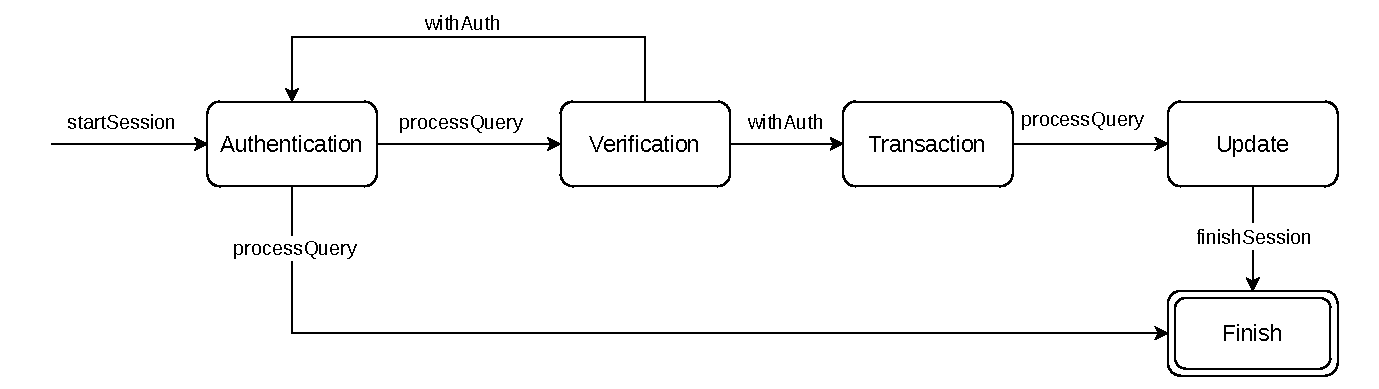
\includegraphics[width=\textwidth, trim={0.8cm 0cm 0.5cm 0cm}, clip]{images/automaton-session.pdf}
    \captionof{figure}{Autómata de una sesión \textit{nano-pop}.}
    \label{fig:automaton-session}
\end{figure}


Con todo esto se puede, finalmente, escribir la lógica principal de una sesión. Ésta se puede encontrar en el módulo \textit{main} del proyecto, junto a la lógica de adquisición de clientes y del \textit{listener socket}.

\vspace{-16pt}
\begin{minipage}[t]{0.48\textwidth}
\begin{lstlisting}[language=Haskell, frame=none, numbers=none, basicstyle=\scriptsize]
-- Gestiona la fase de autorización.
runAuth :: Connection -> Phase Auth -> Reply -> App ()
runAuth conn phase reply = do
  sendReply conn reply

  query <- recvQuery conn

  case processQuery phase query of
    Stay phase' reply' -> runAuth   conn phase' reply'
   Next phase'        -> runVerif  conn phase'
    Term        reply' -> sendReply conn reply'
    Abrt               -> emit Warn "disconnected"

-- Gestiona la fase de verificación. Si withAuth
-- retorna '()', la sesión ha terminado correctamente.
runVerif :: Connection -> Phase Verif -> App ()
runVerif conn auth =
  withAuth auth (runTrans conn) >>= \case
    Left (phase, reply) -> runAuth conn phase reply
    Right ()            -> pure ()
\end{lstlisting}
\vspace{-4pt}
\captionsetup{type=lstlisting}
\caption{Flujo principal de los estados Auth y Verif.}
\end{minipage}
\hfill
\begin{minipage}[t]{0.48\textwidth}
\begin{lstlisting}[language=Haskell, frame=none, numbers=none, basicstyle=\scriptsize, escapechar=|]
-- Gestiona la fase de transacción.
runTrans :: Connection -> Phase Trans -> Reply -> App ()
runTrans conn phase reply = do
  sendReply conn reply

  query <- recvQuery conn

  case processQuery phase query of
    Stay phase' reply' -> runTrans  conn phase' reply'
    Next phase'        -> runUpdate conn phase'
    Term        reply' -> sendReply conn reply'
    Abrt               -> emit Warn "disconnected"

-- Gestiona la fase de actualización y
-- acaba la sesión enviando el mensaje final.
--
-- Nótese que el '()' que devuelve se propaga
-- por todos los estados, finalizando la sesión.
runUpdate :: Connection -> Phase Update -> App ()
runUpdate conn = sendReply conn <=< finishSession
\end{lstlisting}
\vspace{-4pt}
\captionsetup{type=lstlisting}
\caption{Flujo principal de los estados Trans y Update.}
\end{minipage}
\vspace{10pt}

El uso del autómata como estructura central de diseño hace que el flujo de ejecución quede implícitamente determinado por las transiciones entre estados. Como consecuencia, el código gana claridad, ya que cada parte del programa refleja un estado concreto y sus transiciones posibles, y se reduce la probabilidad de errores provocados por transiciones inválidas o casos no contemplados.

%----------------------------------------------------------------------------------------
%   GUÍA DE USO
%----------------------------------------------------------------------------------------

\section{Guía de uso}

Antes de instalar el proyecto, es necesario tener en cuenta algunos requisitos. El sistema de \textit{build} utilizado es \textit{cabal}, por lo que se requiere disponer de \textit{GHC} y \textit{cabal} correctamente instalados en el sistema.

Además, al tratarse de un servidor que depende de \textit{syscalls} del estándar \textit{POSIX}, la aplicación únicamente es compatible con sistemas \textit{Unix}. En sistemas \textit{Windows}, es necesario utilizar una máquina virtual o, de forma más sencilla, ejecutar el proyecto mediante \textit{WSL}.

%----------------------------------------------------------------------------------------

\subsection{Instalación}

Aunque junto a la entrega se proporciona un archivo \texttt{.zip} con el código fuente, el proyecto también puede obtenerse directamente desde el repositorio, que quizás facilita más la instalación. Para compilar e instalar el ejecutable, se deben ejecutar los siguientes comandos desde un terminal ubicado en el directorio deseado:

\vspace{-6pt}
\begin{minipage}{\linewidth}
\begin{lstlisting}[language=bash, numbers=none, basicstyle=\small]
$ git clone https://github.com/suuniqo/npop.git   # clona el repositorio
$ cd npop                                         # entra en el directorio del proyecto
$ cabal build                                     # compila la aplicación
$ cabal install                                   # instala el ejecutable
\end{lstlisting}
\captionsetup{type=lstlisting}
\caption{Instrucciones de instalación a través de un shell.}
\end{minipage}
\vspace{4pt}

Para verificar que la instalación se ha realizado correctamente, se puede comprobar la disponibilidad de los ejecutables \texttt{npop} y \texttt{npop-tools}, generados por el proyecto. Si no se pueden encontrar, el problema seguramente sea que el directorio \texttt{\$HOME/.cabal/bin} no se encuentre en la variable \texttt{\$PATH}. En tal caso, basta con añadir el comando inferior en el fichero de configuración \texttt{.bashrc}:

\vspace{-6pt}
\begin{minipage}{\linewidth}
\begin{lstlisting}[language=bash, numbers=none, basicstyle=\small]
export PATH="$HOME/.cabal/bin:$PATH"
\end{lstlisting}
\captionsetup{type=lstlisting}
\caption{Adición de ejecutables de \textit{cabal} al entorno del \textit{shell}.}
\end{minipage}
\vspace{4pt}

%----------------------------------------------------------------------------------------

\subsection{Configuración}

Una vez instalado, el servidor puede configurarse opcionalmente mediante un archivo \texttt{TOML}. Por defecto, la aplicación busca la configuración en \texttt{\$XDG\_CONFIG\_HOME/npop/config.toml}. Si dicho archivo no existe, se utiliza como alternativa \texttt{\$HOME/.config/npop/config.toml}.

Este fichero permite ajustar tanto parámetros relacionados con la red como opciones de almacenamiento. A continuación se muestran todas las opciones disponibles junto con sus valores por defecto:

\vspace{-6pt}
\begin{minipage}{\linewidth}
\begin{lstlisting}[language={}, numbers=none, basicstyle=\small]
[network]
port           = "pop3"         # puerto o servicio sobre el que escuchar conexiones
idle_timeout   = 600000000      # tiempo máximo de inactividad permitido por cliente
listen_backlog = 16             # número máximo de conexiones pendientes en listen
backoff_min    = 62500          # retardo mínimo usado en exponential backoff
backoff_max    = 16000000       # retardo máximo usado en exponential backoff
read_chunk     = 4096           # bytes leídos en cada operación recv

[storage]
mail_root      = "/var/npop"    # directorio raíz donde se almacenan los buzones
lock_name      = ".lock"        # nombre del fichero utilizado para bloquear buzones
pass_name      = "shadow"       # fichero que contiene las credenciales de usuario
\end{lstlisting}
\captionsetup{type=lstlisting}
\caption{Parámetros configurables con el fichero config.toml.}
\end{minipage}

%----------------------------------------------------------------------------------------

\subsection{Servidor}

Una vez instalado y configurado, el uso del ejecutable principal, \texttt{npop}, es trivial. Basta con ejecutar el comando para iniciar el servicio, que comenzará inmediatamente a aceptar conexiones. Para detenerlo, puede interrumpirse el proceso mediante \texttt{Ctrl-C} o enviando una señal con \textit{kill}.

Dado que se trata de un servicio persistente, lo habitual es ejecutarlo en segundo plano o gestionarlo como un \textit{daemon}. En sistemas \textit{Linux}, la opción recomendada es utilizar \textit{systemd}~\cite{rajpurohit2023systemd}.

\vspace{-6pt}
\begin{minipage}{\linewidth}
\begin{lstlisting}[language=bash, numbers=none, basicstyle=\footnotesize]
$ sudo npop
> npop: ThreadId 1: info: server ready
> npop: ThreadId 2: info: new client: [::1]:56503
> npop: ThreadId 4: warn: client disconnected
> npop: ThreadId 4: info: bye client: [::1]:56503
\end{lstlisting}
\captionsetup{type=lstlisting}
\caption{Ejecución normal del servicio \texttt{npop}.}
\label{lst:npop-correct}
\end{minipage}
\vspace{2pt}

Como puede observarse en el Listing~\ref{lst:npop-correct}, el servidor emite continuamente \textit{logs} con información relevante sobre su ejecución, incluyendo conexiones y desconexiones de clientes, así como eventos anómalos o recuperables.

En caso de producirse un error fatal, el servicio emite el problema y finaliza de forma controlada. Este comportamiento puede observarse en el Listing~\ref{lst:npop-incorrect}:

\vspace{-6pt}
\begin{minipage}{\linewidth}
\begin{lstlisting}[language=bash, numbers=none, basicstyle=\footnotesize]
$ sudo npop
> npop: ThreadId 1: warn: no config file, using defaults
> npop: ThreadId 1: fail: failed to build shadow: /var/npop/shadow: openFile: does not exist (No such file or directory)
\end{lstlisting}
\captionsetup{type=lstlisting}
\caption{Terminación controlada tras un error fatal.}
\label{lst:npop-incorrect}
\end{minipage}
\vspace{2pt}

Primero, se emite un \textit{warning} al no encontrarse el fichero de configuración, situación recuperable en la que se utilizan los valores por defecto. Posteriormente, se produce un fallo irrecuperable al no localizar el fichero de autenticación \texttt{shadow}.

Nótese además la cantidad de contexto adicional incorporado a los mensajes de error gracias el \textit{wrapper} \texttt{SysErr} y el módulo de \textit{logging}, incluyendo el hilo responsable y la operación que provocó el fallo.

Cabe destacar también, que el fichero \texttt{shadow} posee permisos restringidos. Por este motivo, el servicio debe ejecutarse con \texttt{sudo} para poder acceder a él. En caso contrario, se produce el siguiente error: 

\vspace{-6pt}
\begin{minipage}{\linewidth}
\begin{lstlisting}[language=bash, numbers=none, basicstyle=\footnotesize]
$ npop
> npop: ThreadId 1: fail: failed to build shadow: /var/npop/shadow: openFile: permission denied (Permission denied)
\end{lstlisting}
\captionsetup{type=lstlisting}
\caption{Error de permisos al acceder al fichero \texttt{shadow}.}
\end{minipage}

%----------------------------------------------------------------------------------------

\subsection{Cliente}

Aunque en esta práctica no se ha desarrollado un cliente \texttt{POP3}, se puede interactuar con el servicio fácilmente con \texttt{telnet} o \texttt{netcat}. Para ello, basta con conectarse al puerto del servidor e introducir los comandos manualmente:

\vspace{-16pt}
\begin{minipage}[t]{0.48\textwidth}
\begin{lstlisting}[language={}, numbers=none, basicstyle=\footnotesize]
$ telnet localhost pop3
> +OK POP3 server ready
> user bob
> +OK
> pass admin
> +OK bob's maildrop has 3 messages (994 octets)
> stat
> +OK 3 994
> list
> +OK
> 1 374
> 2 332
> 3 288
> .
> retr 1
> +OK 374 octets
> From: alice@example.com
> To: bob@local
> Subject: Greeting 
> 
> Hi Bob,
> Just wanted to say hi.
> Alice
> .
> quit
> +OK POP3 server signing off (3 messages left)
\end{lstlisting}
\vspace{-4pt}
\captionsetup{type=lstlisting}
\caption{Sesión POP3 correcta, usando telnet.}
\end{minipage}
\hfill
\begin{minipage}[t]{0.49\textwidth}
\begin{lstlisting}[language=Haskell, numbers=none, basicstyle=\footnotesize]
$ nc -c ::1 110
> +OK POP3 server ready
> user alice
> +OK
> pass qwerty
> -ERR invalid credentials
> USER alice
> +OK
> PaSs admin
> +OK alice's maildrop has 3 messages (994 octets)
> download 1
> -ERR unknown command
> retr 14
> -ERR no such message
> dele 1
> +OK message 1 deleted
> dele 1
> -ERR message already deleted
> rset
> +OK restored 1 messages (374 octets)
> aaaaaaaaaaaaaaaaaaaaaaaaaaaaaaaaaaaaaaaaaaaaaa
> -ERR query is too long
>
> -ERR empty query
> quit
> +OK POP3 server signing off (3 messages left)
\end{lstlisting}
\vspace{-4pt}
\captionsetup{type=lstlisting}
\caption{Sesión POP3 con errores, usando netcat.}
\end{minipage}

%----------------------------------------------------------------------------------------

\subsection{Herramientas}

Finalmente, para facilitar la gestión de usuarios en \textit{Maildir}, así como su autenticación, se ha creado el \textit{script} \texttt{npop-tools}, que automatiza todas estas tareas. Existren tres modos de uso:

\begin{tabular}{l@{\hspace{3pt}} c@{\hspace{3pt}}l@{\hspace{8pt}}l l}
    \texttt{\textbf{npop-tools}} & \texttt{\textbf{add}} & \texttt{\textbf{user:}} &
    Crea tanto la entrada en \textit{shadow}, como los directorios \textit{Maildir}, del usuario provisto. \\

    \texttt{\textbf{npop-tools}} & \texttt{\textbf{del}} & \texttt{\textbf{user:}} &
    Elimina la entrada en \textit{shadow} y los directorios \textit{Maildir} del usuario provisto. \\ 

    \texttt{\textbf{npop-tools}} & \texttt{\textbf{put}} & \texttt{\textbf{user:}} &
    Introduce un mensaje en el buzón del usuario provisto, usando el formato correcto. \\
\end{tabular}

De nuevo, es necesario utilizar \texttt{sudo} para ejecutar los comandos que modifican el fichero \textit{shadow}.

\vspace{-20pt}
\begin{minipage}[t]{0.29\textwidth}
\begin{lstlisting}[language=Haskell, numbers=none, basicstyle=\footnotesize]
$ sudo npop-tools add alice
> password:
> npop-tools: added user alice
\end{lstlisting}
\vspace{-4pt}
\captionsetup{type=lstlisting}
\caption{Añadir el usuario Alice.}
\end{minipage}
\hfill
\begin{minipage}[t]{0.31\textwidth}
\begin{lstlisting}[language=Haskell, numbers=none, basicstyle=\footnotesize, escapechar=|]
$ sudo npop-tools del alice
> npop-tools: deleted user alice
|
\end{lstlisting}
\vspace{-4pt}
\captionsetup{type=lstlisting}
\caption{Borrar el usuario Alice.}
\end{minipage}
\hfill
\begin{minipage}[t]{0.35\textwidth}
\begin{lstlisting}[language=Haskell, numbers=none, basicstyle=\footnotesize]
$ npop-tools put alice
> message: hey alice!^D
> npop-tools: sent message to alice
\end{lstlisting}
\vspace{-4pt}
\captionsetup{type=lstlisting}
\caption{Mandar un mensaje a Alice.}
\end{minipage}

%----------------------------------------------------------------------------------------
%   VALIDACIÓN DEL SISTEMA
%----------------------------------------------------------------------------------------

%----------------------------------------------------------------------------------------
%   VALIDACIÓN DEL SISTEMA
%----------------------------------------------------------------------------------------

\section{Validación del sistema}

Con el objetivo de garantizar la corrección y robustez del servidor, se han realizado dos tipos principales de pruebas. Por un lado, pruebas programáticas sobre los módulos internos más críticos de la aplicación. Por otro, pruebas de integración mediante clientes \texttt{POP3} reales, con el fin de verificar el comportamiento del servidor en escenarios de uso reales y su compatibilidad con el protocolo.

%----------------------------------------------------------------------------------------

\subsection{Pruebas programáticas}

Las pruebas programáticas se han centrado en los dos módulos más propensos a errores: el \textit{parser} de consultas \texttt{POP3} y el módulo de almacenamiento.

El módulo de \textit{parsing} es uno de los más propensos a errores en cualquier aplicación, ya que el procesamiento de entradas externas suele ser especialmente delicado y fácil de implementar de forma incorrecta. Por suerte, los comandos \texttt{POP3} siguen una gramática bastante sencilla:

\begin{center}
    \texttt{<ESPACIADO> <COMANDO> <ESPACIADO> [<ARGUMENTO> <ESPACIADO>]}
\end{center}

Dado que la longitud máxima de una consulta es de 45 caracteres, resulta viable generar y comprobar un gran número de casos de forma automática. Para ello se ha utilizado \textit{fuzzing} mediante la librería \textit{Hedgehog}, generando tanto consultas válidas como inválidas y verificando propiedades como la insensibilidad a mayúsculas, la tolerancia al espaciado o la correcta detección de errores en entradas malformadas.

Por otro lado, el módulo de almacenamiento requiere especial fiabilidad, ya que interpreta buzones en formato \textit{Maildir}, extrae los mensajes con sus banderas y serializa buzones virtuales sobre el sistema de ficheros. Su validación es muy importante para garantizar la consistencia de los datos y evitar pérdidas o corrupciones.

En este caso se han utilizado principalmente \textit{unit tests} mediante la librería \textit{HSpec}. Estas pruebas operan sobre directorios temporales donde se ejecutan operaciones reales de lectura y escritura, comprobando finalmente que el estado del buzón coincide con el esperado.

%----------------------------------------------------------------------------------------

\subsection{Pruebas de integración}

Las pruebas de integración se han realizado con clientes reales para validar no solo la corrección del protocolo, sino también la interoperabilidad del servidor con implementaciones ampliamente utilizadas. Se han utilizado herramientas con distintos patrones de uso para detectar posibles desviaciones del estándar y problemas de implementación que no aparecen en pruebas unitarias.

\vspace{-12pt}
\begin{minipage}[t]{0.50\textwidth}
\begin{lstlisting}[language={}, numbers=none, basicstyle=\scriptsize]
$ fetchmail -v -p POP3 -P 110 -u bob
POP3< +OK POP3 server ready
POP3> CAPA
POP3< +OK
POP3< USER
POP3< .
POP3> USER bob
POP3< +OK
POP3> PASS *
POP3< +OK bob's maildrop has 1 messages (374 octets)
POP3> STAT
POP3< +OK 1 374
1 message for bob at localhost (374 octets).
POP3> LIST 1
POP3< +OK 1 374
POP3> RETR 1
POP3< +OK 374 octets
reading message bob@localhost:1 of 1 (374 octets) flushed
POP3> DELE 1
POP3< +OK message 1 deleted
POP3> QUIT
POP3< +OK POP3 server signing off (maildrop empty)
6.6.4 querying localhost (protocol POP3): poll completed
normal termination, status 0
\end{lstlisting}
\vspace{-4pt}
\captionsetup{type=lstlisting}
\caption{Integración con un cliente \textit{fetchmail}}
\end{minipage}
\hfill
\begin{minipage}[t]{0.45\textwidth}
\begin{lstlisting}[language={}, numbers=none, basicstyle=\scriptsize]
$ curl -v pop3://localhost:110/1 --user "bob:admin"
* Connected to localhost (::1) port 110
< +OK POP3 server ready
> CAPA
< +OK
< USER
< .
> USER bob
< +OK
> PASS admin
< +OK bob's maildrop has 1 messages (39 octets)
> RETR 1
< +OK 39 octets
From: alice@example.com
To: bob@local
Subject: Project Update
Date: Mon, 4 May 2026 09:00:00 +0000

Hi Bob,

I just wanted to say hi.

Alice
* Connection #0 to host localhost left intact
\end{lstlisting}
\vspace{-4pt}
\captionsetup{type=lstlisting}
\caption{Integración con un cliente \textit{curl}}
\end{minipage}

%----------------------------------------------------------------------------------------
%   CONCLUSIÓN
%----------------------------------------------------------------------------------------

\section{Conclusión}

El diseño del servidor utilizando el patrón \textit{typestate} para modelar el autómata de estados de una sesión \texttt{POP3} ha resultado especialmente exitoso. Representar las fases del protocolo directamente en el sistema de tipos ha permitido simplificar considerablemente la lógica del flujo principal del programa, eliminando gran cantidad de comprobaciones manuales y trasladando muchas restricciones al compilador.

Además de mejorar la claridad del código, este enfoque ha contribuido de forma directa a aumentar la robustez y fiabilidad del sistema. Las transiciones inválidas entre estados quedan imposibilitadas a nivel de tipos, reduciendo errores lógicos difíciles de detectar y facilitando el mantenimiento del código. En combinación con una gestión estructurada de excepciones y una liberación segura de recursos mediante \texttt{bracket}, el resultado es un servidor razonablemente tolerante a fallos incluso en presencia de errores inesperados.

No obstante, el proyecto presenta todavía varias limitaciones importantes. La más relevante es la ausencia de cifrado en las comunicaciones. Actualmente, las credenciales de autenticación se transmiten en \textit{plaintext} a través de la red, lo que supone un problema grave de seguridad en entornos reales. La solución adecuada sería utilizar \texttt{TLS}, permitiendo establecer conexiones cifradas entre cliente y servidor. Sin embargo, debido a la complejidad adicional que introduce y al alcance del proyecto, esta funcionalidad no se ha implementado.

Por otro lado, el servidor tampoco incorpora mecanismos específicos de defensa frente a clientes maliciosos. Por ejemplo, un cliente puede enviar \textit{queries} incorrectos infinitamente, haciendo el servidor susceptible a ataques \textit{DDoS}. Sería recomendable añadir límites de intentos fallidos de autenticación y sistemas de expulsión de clientes.

%----------------------------------------------------------------------------------------
%   BIBLIOGRAFÍA
%----------------------------------------------------------------------------------------

\printbibliography

%----------------------------------------------------------------------------------------

\end{document}
